% Generated by paper/src/render.py from main_text.py; edit the source, not this file.
\documentclass[numsec,webpdf,modern,large]{oup-authoring-template}
\usepackage{booktabs}
\newcommand{\dinara}{dinara-align}
\tikzset{
  dinara/.style={very thick, black},
  apafull/.style={thick, blue!80!black},
  apasimple/.style={thick, cyan!70!black, dashed},
  apa/.style={thick, violet, dotted},
  edlib/.style={thick, orange!85!black},
  biwfa/.style={thick, red!75!black, dashed},
  wfa/.style={thick, green!50!black},
  quicked/.style={thick, brown!70!black, dash dot},
}

\begin{document}
\journaltitle{Bioinformatics}
\DOI{DOI added during production}
\copyrightyear{2026}
\pubyear{2026}
\access{Published: Date added during production}
\appnotes{Original Paper}
\firstpage{1}
\title[dinara-align]{dinara-align: hardware-aware algorithms for exact pairwise alignment}
\author[1,$\ast$]{Konstantinos Kyriakidis}
\author[1,$\ast$]{Benedict Paten}
\address[1]{\orgname{UC Santa Cruz Genomics Institute}, \orgaddress{\state{Santa Cruz, CA}, \country{USA}}}
\corresp[$\ast$]{Corresponding authors. \href{mailto:kkyriaki@ucsc.edu}{kkyriaki@ucsc.edu}, \href{mailto:bpaten@ucsc.edu}{bpaten@ucsc.edu}}
\received{Date}{0}{Year}
\revised{Date}{0}{Year}
\accepted{Date}{0}{Year}
\abstract{\textbf{Motivation:} Exact pairwise alignment returns an optimal alignment that no heuristic cut-off can change, the reference for evaluating read mappers, assemblers and variant callers. Yet no exact algorithm is fastest across workloads: diagonal transition wins on near-identical pairs, bit-parallel band doubling on long divergent reads, and inter-sequence vectorisation on batches of short pairs.\\
\textbf{Results:} We present dinara-align, an exact aligner that chooses its algorithm for each pair. Every hand-over that rests on a projection provably bounds its waste; a gap-affine alignment adds a second search only when its measured work exceeds what two would need, provably still finding an optimal alignment; short pairs are aligned in bands that each vector lane certifies optimal; and, within the memory limit, all engines break ties alike at unit and gap-affine costs. On one Skylake-X core, dinara-align was the fastest exact aligner compared on every dataset at unit costs: up to 2.4 times faster than A*PA2 on ultra-long nanopore reads, and 1.9 and 5.1 times faster than WFA on Illumina and HiFi reads. At gap-affine costs it was the fastest on every dataset any tool completed, tied with WFA on Illumina reads.\\
\textbf{Availability and implementation:} dinara-align is free software under the Mozilla Public License 2.0, available at \url{https://github.com/kokyriakidis/dinara-align} with C, C++, Python and command-line interfaces.}
\keywords{pairwise alignment, edit distance, gap-affine alignment, band doubling, diagonal transition, SIMD}
\maketitle
\section{Introduction}

Pairwise alignment finds the least costly series of substitutions, insertions and deletions that transforms one sequence into another. It underlies read mapping, variant detection, genome assembly and multiple sequence alignment \citep{Prjibelski2019sequence}: read mappers align each read to the reference window its seeds select, assemblers compare reads with one another to find their overlaps \citep{Li2018minimap2}, and assemblies, haplotypes and viral genomes are compared base by base.

Read lengths have grown from hundreds of bases to hundreds of kilobases. The gap-affine dynamic program \citep{Gotoh1982} fills an \(n \times m\) matrix, \(2.5 \times 10^{11}\) cells for one pair of 500~kbp reads, so heuristic aligners compute only part of it: a fixed or adaptive band \citep{Liu2023blockaligner}, a series of windows, or the cells before the score drops by more than a threshold (X-drop, or Z-drop in minimap2 \citep{Li2018minimap2}). Their result then depends on these cut-offs, and alignments with large indels or clustered errors can be missed or misplaced. Exact aligners instead skip only cells that provably cannot lie on an optimal path, so that their running time grows with the distance as well as the length, rather than with the product of the lengths.

Three ideas underlie current exact aligners. \emph{Band doubling} computes only the diagonals a path within a cost bound can reach, doubling the bound until the optimum lies within it \citep{Ukkonen1985}; \emph{bit-parallelism} encodes the score differences of 64 cells of a column in two machine words \citep{Myers1999bitvector}, and Edlib combines the two \citep{Sosic2017edlib}. \emph{Diagonal transition} extends the furthest-reaching paths one cost at a time \citep{Ukkonen1985,Myers1986ond}; WFA extended it to gap-affine costs \citep{MarcoSola2021wfa} and BiWFA made its memory linear in the distance \citep{MarcoSola2023biwfa}. A*PA guided an A* search by a gap-chaining seed heuristic \citep{GrootKoerkamp2024astarpa}; A*PA2 combined that heuristic with band doubling over SIMD blocks, aligning ultra-long reads up to 19 times faster than Edlib and BiWFA \citep{GrootKoerkamp2024astarpa2}; and QuickEd aligns within a bound it finds heuristically \citep{Doblas2025quicked}. Full-matrix vectorisation, in anti-diagonal \citep{Wozniak1997}, striped \citep{Farrar2007striped,Zhao2013ssw}, prefix-scan \citep{Daily2016parasail}, difference-recurrence \citep{Suzuki2018diff,Li2018minimap2} and inter-sequence \citep{Rognes2011swipe,Rahn2018seqan} layouts, takes time in proportion to the matrix or the band instead.

Each of these methods is fastest on part of the range of workloads: diagonal transition, whose expected work grows with the square of the distance, on short and near-identical pairs; bit-parallel band doubling, whose work grows with the length times the distance, on long divergent reads, with the seed heuristic on ultra-long ones; and inter-sequence vectorisation on batches of short pairs. An aligner that is fastest across workloads must therefore choose among them for each pair, and an exact aligner must make every such choice (which algorithm, which bound, when to abandon a search) without giving up optimality. In dinara-align every engine is exact, so no choice changes the optimal cost, and every hand-over that rests on a projection provably bounds the work it can waste. Our contributions are:

\begin{enumerate}
  \item \textbf{One wavefront search or two, chosen by measured work} (Section 3.9): a gap-affine alignment adds a second search only when its measured work exceeds what two would need, and still returns an optimal alignment (Proposition 2).
  \item \textbf{Projections with bounded waste} (Sections 3.3 and 3.10): a projected distance sets a band's first bound only when two projections agree, and a search hands over to an algorithm projected to be cheaper only after spending one twenty-fourth of that algorithm's least possible work.
  \item \textbf{Certified bands for inter-sequence batches} (Section 3.6): each pair is aligned in a vector lane within a narrow band that the lane certifies optimal under gap-affine and two-piece costs (Proposition 1), bringing the speculate-and-verify approach of narrow-band aligners \citep{Gibrat2018band,Fujiki2020seedex} to every lane of a batch.
  \item \textbf{Direct neighbour construction for the seed heuristic} (Section 3.5): inexact neighbours of exact seed matches are inserted without search, provably including every one that local pruning keeps (Lemma 1); we also prove that A*PA2's pruning keeps the heuristic a lower bound (Lemma S1).
  \item \textbf{One alignment whichever engine computes it} (Sections 3.1 and 3.7): at unit, gap-affine and two-piece costs every engine breaks ties by the same rule, unless a gap-affine pair must be split to fit the memory limit, and a unit-cost band recomputes its traceback from recorded state rather than splitting the pair, so that its alignment is the same under any memory limit.
  \item \textbf{Engines arranged for the processor} (Sections 3.2, 3.4 and 3.11): diagonal transition with gathered AVX-512 loads, interleaved bit-parallel groups with a shorter dependency chain, and lower per-pair overhead on short reads.
  \item \textbf{One library} (Table~\ref{tab:engines}; Supplementary Table S3) for global, ends-free, extension and local alignment under unit, gap-affine, two-piece and substitution-matrix costs, for single pairs and batches, through C, C++, Python and command-line interfaces.
\end{enumerate}

We evaluate dinara-align on the datasets of the A*PA2 and QuickEd benchmarks, with QuickEd's Illumina, HiFi and PromethION sets built from HG002 reads, each paired with the stretch of HG002's own assembly it covers.

\section{Background}

\subsection{Alignment and costs}

Let \(A=a_1\dots a_n\) be the reference and \(B=b_1\dots b_m\) the query, and let cell \((i,j)\) lie on diagonal \(j-i\). Under gap-affine costs \((x, o, e)\), for example (4, 6, 2), a match costs 0, a mismatch \(x\) and a gap of \(k\) letters \(g(k)=o+ke\); unit costs have \(x=e=1\) and \(o=0\), two-piece costs take the minimum of two such functions \citep{Li2018minimap2}, and a substitution matrix instead scores each pair of letters. Global alignment compares two whole sequences; ends-free alignment places a read inside a longer window or finds the overlap of two reads; extension grows an alignment from a seed match \citep{Li2018minimap2}; and local alignment finds the best-matching parts of two sequences. Extension and local alignment maximise a score that rewards each match (Section 3.8). An alignment is \emph{optimal} if no alignment has lower cost under the requested costs and mode; a caller may further restrict alignments to a band of diagonals or a maximum cost, and an exact aligner then returns an optimal alignment among those or reports that none exists. At unit costs the distance \(D(i,j)\) between the prefixes \(a_1\dots a_i\) and \(b_1\dots b_j\) satisfies

\begin{equation}\begin{gathered}
D(i,j) = \min\bigl(D(i-1,j)+1,\; D(i,j-1)+1,\\ D(i-1,j-1)+[a_i \ne b_j]\bigr),
\end{gathered}\end{equation}

where \([a_i \ne b_j]\) is 1 if the letters differ and 0 otherwise, with \(D(i,0)=i\) and \(D(0,j)=j\), and the distance is \(D(n,m)\); gap-affine costs need three such layers \citep{Gotoh1982}.

\subsection{Band doubling and bit-parallel computation}

At unit costs, an alignment of cost at most \(t\) visits only diagonals \(d\) with \(|d| + |d - \delta| \le t\), where \(\delta = m - n\); band doubling computes only those cells, doubling \(t\) until \(D(n,m) \le t\) \citep{Ukkonen1985}. Myers' recurrence advances the score differences of 64 cells of a column, held in two machine words, by one column at a time \citep{Myers1999bitvector}, and A*PA2 computes the band in tiles of 256 columns with SIMD vectors \citep{GrootKoerkamp2024astarpa2}.

\subsection{Diagonal transition}

Diagonal transition keeps, for each cost \(s\) and diagonal, the furthest cell an alignment of cost \(s\) reaches, extended along matches at no cost, in \(O(ns)\) time in the worst case and \(O(n + s^2)\) expected time on random sequences \citep{Ukkonen1985,Myers1986ond}; WFA generalises it to gap-affine costs, where the wavefront, or front, of each cost has three layers \citep{MarcoSola2021wfa}, and BiWFA runs it from both ends \citep{MarcoSola2023biwfa}.

\subsection{The seed heuristic}

A*PA divides the reference into disjoint seeds of fixed length and finds their matches in the query, exactly or with one edit \citep{GrootKoerkamp2024astarpa}. The potential of a seed is the cost \(r\) of crossing it unmatched, 1 for exact seeds and 2 for seeds matched with one edit, and a match crosses a seed for less than \(r\). The gap-chaining seed heuristic charges a chain of matches from a cell the cost of each match and, for each gap between consecutive matches and from the last to the end, the larger of the potential of the seeds that start in the gap and the number of diagonals it shifts. Its value, the least charge of any chain, never exceeds the remaining cost, and A*PA keeps the match starts in layers by the value of the best chain each begins \citep{GrootKoerkamp2024astarpa}. A*PA2 prunes matches before the alignment, in place of A*PA's pruning during the search: a match \(\nu\) with cost \(c(\nu)\) and end cell \(\mathrm{end}(\nu)\) is kept only if a path from \(\mathrm{end}(\nu)\), starting at cost \(c(\nu)\), crosses the next \(p = 14\) seeds, counting that of \(\nu\), while its cost stays below the potential of the seeds it has crossed \citep{GrootKoerkamp2024astarpa2}. A diagonal transition from \(\mathrm{end}(\nu)\) tests this, dropping each furthest-reaching point whose cost reaches that potential; a further point on a diagonal has crossed at least as much potential, so no such path is missed. A*PA2 uses the heuristic to drop the rows of each band whose score plus the heuristic exceeds the bound \citep{GrootKoerkamp2024astarpa2}.

\section{Methods}

\subsection{Overview}

Each problem is assigned to an algorithm (Table~\ref{tab:engines}; Fig.~\ref{fig:overview}). Unit costs follow A*PA2 \citep{GrootKoerkamp2024astarpa2}: band doubling over 256-column tiles of bit-parallel words, pruned on long pairs by the gap-chaining seed heuristic \citep{GrootKoerkamp2024astarpa}, with near-identical pairs aligned by diagonal transition alone. Gap-affine costs use the wavefront of WFA and BiWFA \citep{MarcoSola2021wfa,MarcoSola2023biwfa}. At unit costs, diagonal transition runs first and hands over once its projected remaining work exceeds the alternative's and it has spent a twenty-fourth of it (Section 3.10); its projection, the length and the cost model then choose the next algorithm and its parameters.

At unit, gap-affine and two-piece costs, every engine selects the same alignment among equally good ones, by the backtrace order of WFA2-lib: from the end, an edit into a cell is preferred to a match whenever one is optimal, a substitution before a deletion (a letter of \(A\) alone) before an insertion (a letter of \(B\) alone), the second gap piece before the first, and a gap extended before it is opened. This rule gives WFA2-lib's CIGARs exactly; the default applies it to both sequences reversed, which places every edit as far left as possible, as variant callers normalise indels. The wavefronts and the tile traceback (Section 3.4) take the furthest-reaching source, which makes the same choice, and the batches and the difference sweep store per-cell flags under the rule. Two exceptions remain: a gap-affine pair whose wavefronts would exceed the memory limit is split and follows the rule within each piece, and alignments under a substitution matrix follow the traceback order of Gotoh's recurrence.

\begin{figure*}[t]
\centering
\resizebox{\textwidth}{!}{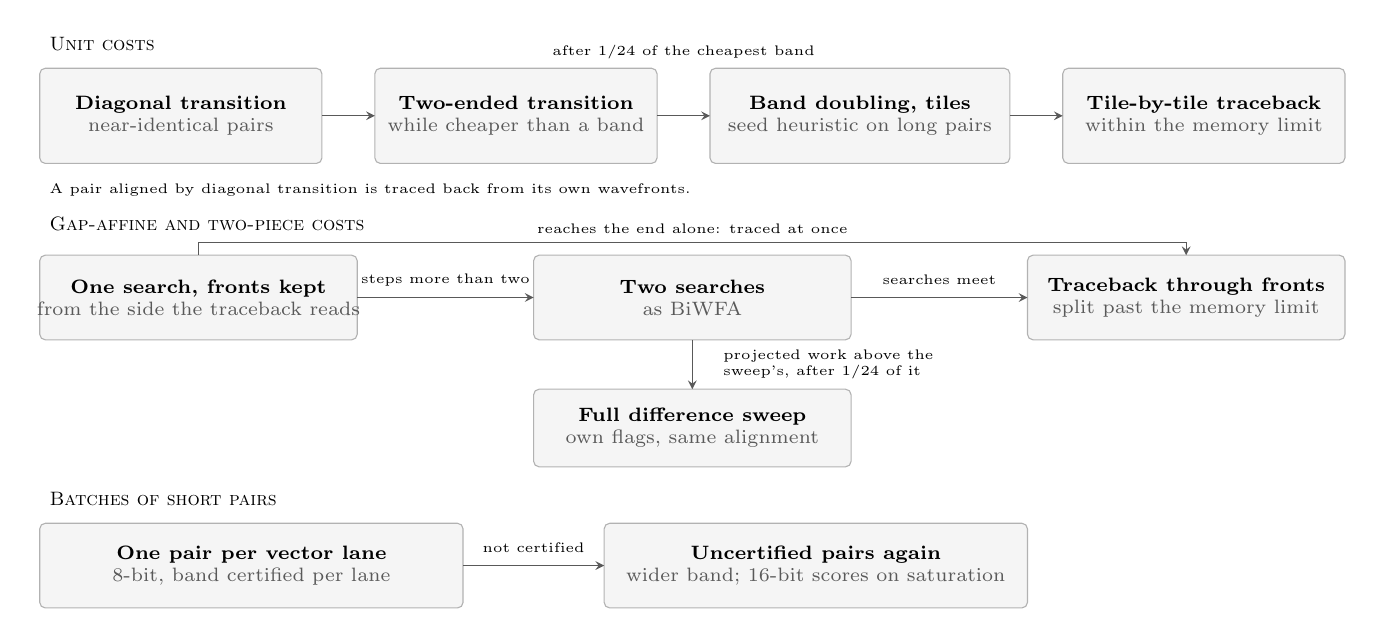
\begin{tikzpicture}
\node[anchor=west,font=\scriptsize\scshape] at (0.224,-0.224) {Unit costs};
\node[anchor=west,font=\scriptsize\scshape] at (0.224,-2.509) {Gap-affine and two-piece costs};
\node[anchor=west,font=\scriptsize\scshape] at (0.224,-6.003) {Batches of short pairs};
\draw[rounded corners=2pt,fill=gray!8,draw=gray!60] (0.224,-0.538) rectangle (3.808,-1.747);
\node[align=center,font=\scriptsize] at (2.016,-1.142) {\textbf{Diagonal transition}\\{\color{gray!70!black}near-identical pairs}};
\draw[rounded corners=2pt,fill=gray!8,draw=gray!60] (4.480,-0.538) rectangle (8.064,-1.747);
\node[align=center,font=\scriptsize] at (6.272,-1.142) {\textbf{Two-ended transition}\\{\color{gray!70!black}while cheaper than a band}};
\draw[rounded corners=2pt,fill=gray!8,draw=gray!60] (8.736,-0.538) rectangle (12.544,-1.747);
\node[align=center,font=\scriptsize] at (10.640,-1.142) {\textbf{Band doubling, tiles}\\{\color{gray!70!black}seed heuristic on long pairs}};
\draw[rounded corners=2pt,fill=gray!8,draw=gray!60] (13.216,-0.538) rectangle (16.800,-1.747);
\node[align=center,font=\scriptsize] at (15.008,-1.142) {\textbf{Tile-by-tile traceback}\\{\color{gray!70!black}within the memory limit}};
\draw[rounded corners=2pt,fill=gray!8,draw=gray!60] (0.224,-2.912) rectangle (4.256,-3.987);
\node[align=center,font=\scriptsize] at (2.240,-3.450) {\textbf{One search, fronts kept}\\{\color{gray!70!black}from the side the traceback reads}};
\draw[rounded corners=2pt,fill=gray!8,draw=gray!60] (6.496,-2.912) rectangle (10.528,-3.987);
\node[align=center,font=\scriptsize] at (8.512,-3.450) {\textbf{Two searches}\\{\color{gray!70!black}as BiWFA}};
\draw[rounded corners=2pt,fill=gray!8,draw=gray!60] (12.768,-2.912) rectangle (16.800,-3.987);
\node[align=center,font=\scriptsize] at (14.784,-3.450) {\textbf{Traceback through fronts}\\{\color{gray!70!black}split past the memory limit}};
\draw[rounded corners=2pt,fill=gray!8,draw=gray!60] (6.496,-4.614) rectangle (10.528,-5.600);
\node[align=center,font=\scriptsize] at (8.512,-5.107) {\textbf{Full difference sweep}\\{\color{gray!70!black}own flags, same alignment}};
\draw[rounded corners=2pt,fill=gray!8,draw=gray!60] (0.224,-6.317) rectangle (5.600,-7.392);
\node[align=center,font=\scriptsize] at (2.912,-6.854) {\textbf{One pair per vector lane}\\{\color{gray!70!black}8-bit, band certified per lane}};
\draw[rounded corners=2pt,fill=gray!8,draw=gray!60] (7.392,-6.317) rectangle (12.768,-7.392);
\node[align=center,font=\scriptsize] at (10.080,-6.854) {\textbf{Uncertified pairs again}\\{\color{gray!70!black}wider band; 16-bit scores on saturation}};
\draw[->,>=stealth,gray!70!black] (3.808,-1.142) -- (4.480,-1.142);
\draw[->,>=stealth,gray!70!black] (8.064,-1.142) -- (8.736,-1.142);
\node[align=center,font=\tiny] at (8.400,-0.336) {after 1/24 of the cheapest band};
\draw[->,>=stealth,gray!70!black] (12.544,-1.142) -- (13.216,-1.142);
\draw[->,>=stealth,gray!70!black] (4.256,-3.450) -- (6.496,-3.450);
\node[align=center,font=\tiny] at (5.376,-3.226) {steps more than two};
\draw[->,>=stealth,gray!70!black] (10.528,-3.450) -- (12.768,-3.450);
\node[align=center,font=\tiny] at (11.648,-3.226) {searches meet};
\draw[->,>=stealth,gray!70!black] (2.240,-2.912) -- (2.240,-2.755) -- (14.784,-2.755) -- (14.784,-2.912);
\node[align=center,font=\tiny] at (8.512,-2.576) {reaches the end alone: traced at once};
\draw[->,>=stealth,gray!70!black] (8.512,-3.987) -- (8.512,-4.614);
\node[anchor=west,align=left,font=\tiny] at (8.781,-4.301) {projected work above the\\sweep's, after 1/24 of it};
\draw[->,>=stealth,gray!70!black] (5.600,-6.854) -- (7.392,-6.854);
\node[align=center,font=\tiny] at (6.496,-6.630) {not certified};
\node[anchor=west,font=\tiny] at (0.224,-2.083) {A pair aligned by diagonal transition is traced back from its own wavefronts.};
\end{tikzpicture}}
\caption{How dinara-align assigns a pair to an algorithm, and the rule behind each hand-over. At unit costs, diagonal transition from one end and then from both aligns near-identical pairs, handing over to band doubling over bit-parallel tiles only once its projected work exceeds the band's and it has spent one twenty-fourth of the cheapest band (Section 3.10); the tiles are traced back within the memory limit. At gap-affine costs one search grows alone, its fronts kept, and is traced back at once if it reaches the end; a second search joins once one would step more diagonals than two would need (Section 3.9), and a global pair projected to take more work than a full sweep in difference recurrences is handed to that sweep after one twenty-fourth of its work, the alignment the same either way. Batches of short pairs are aligned one pair per vector lane within a band whose optimality each lane certifies (Section 3.6). The figure shows alignments; a unit-cost distance skips the one-ended search.}\label{fig:overview}
\end{figure*}

\begin{table*}[t]
\caption{Algorithms in dinara-align and the changes introduced in this work.}\label{tab:engines}
\centering\footnotesize
\setlength{\tabcolsep}{4pt}
\begin{tabular}{@{}l>{\raggedright\arraybackslash}p{5.2cm}>{\raggedright\arraybackslash}p{5.2cm}@{}}
\toprule
Problem & Algorithm & Changes (section) \\
\midrule
Unit costs, divergent pairs & Band doubling over bit-parallel tiles with the gap-chaining seed heuristic (A*PA2) & Regrouped recurrence, interleaved groups (3.2); agreeing estimates (3.3); direct neighbours (3.5); traceback within a memory limit (3.7) \\
Unit costs, near-identical pairs & Diagonal transition (WFA, BiWFA) & Gathered extension (3.4); bounded-waste hand-over (3.10); per-pair overhead (3.11) \\
Gap-affine, two-piece & Wavefront, one search or two (WFA, BiWFA); full sweep in difference recurrences for divergent pairs (Suzuki and Kasahara, 2018) & Gathered extension (3.4); one search or two (3.9); bounded-waste hand-over (3.10) \\
Substitution matrices & Anti-diagonal vector sweep (Wozniak, 1997) & Score-certified band, cache-sized strips (3.8) \\
Local alignment & End found by a forward sweep (Zhao et al., 2013) & Backward wavefront from the best end (3.8) \\
Batches of short pairs & Inter-sequence vectorisation (Rognes, 2011; Rahn et al., 2018; Daily, 2016) & Certified per-lane bands (3.6) \\
\bottomrule
\end{tabular}
\end{table*}

\subsection{A shorter critical path for Myers' recurrence}

As in Edlib and A*PA2 \citep{Sosic2017edlib,GrootKoerkamp2024astarpa2}, the query is packed 64 bases per word, and Myers' recurrence \citep{Myers1999bitvector} advances a word by one column. With match mask \(E\), vertical difference masks \(P_v, M_v\) and the incoming negative horizontal difference folded into \(E' = E \lor M_h^{\mathrm{in}}\), A*PA2 computes

\begin{equation}\begin{gathered}
c = (E' \land P_v) + P_v,\\ X_h = (c \oplus P_v) \lor E',\\ P_h = M_v \lor \lnot(X_h \lor P_v),\\ M_h = P_v \land X_h.
\end{gathered}\end{equation}

The horizontal masks \(P_h\) and \(M_h\) determine the vertical masks of the next column, so the path from \(c\) to them lies on the loop-carried chain. Since \((c \oplus P_v) \lor P_v = c \lor P_v\) and \(P_v \land (c \oplus P_v) = P_v \land \lnot c\), the same masks are obtained as

\begin{equation}\begin{gathered}
P_h = M_v \lor \lnot\bigl(c \lor (E' \lor P_v)\bigr),\\ M_h = (P_v \land \lnot c) \lor (P_v \land E'),
\end{gathered}\end{equation}

where \(E' \lor P_v\) and \(P_v \land E'\) do not depend on \(c\) and are computed off the critical path. The vertical update is regrouped in the same way, its negated part computed from \(E\), \(M_v\) and the incoming horizontal difference before \(P_h\) is known. Together the rewrites shorten the loop-carried chain of a single word from 14 to 8 cycles per column. \citet{Myers1999bitvector}, Edlib and A*PA2 use the original form, and we are not aware of a previous description of the regrouped one.

Words occupy the lanes of a vector, staggered by one column, so that the horizontal difference leaving one word enters the next through a lane rotation \citep{Wozniak1997,GrootKoerkamp2024astarpa2}, and each column waits for the rotation of the previous one. A*PA2 overlaps these waits with two four-lane vectors; on AVX-512, where a vector holds eight words, dinara-align interleaves two eight-word groups, the lower ten columns behind the upper, so that each fills the latency of the other. Bands of two or three words run in general-purpose registers, whose operations have lower latency.

\subsection{Band bounds from agreeing estimates}

Band doubling is exact for any initial bound, but its running time depends on how close that bound is to the distance. A computation that has reached cost \(s\) at anti-diagonal \(\rho\) estimates the distance as \(\hat D = s(n+m)/\rho\), which is reliable when edits are spread evenly and too high by orders of magnitude when they gather, as at the ends of nanopore reads. dinara-align therefore takes two estimates, \(\hat D_1\) from a one-ended diagonal-transition search stopped after eight edits and \(\hat D_2\) from the two-ended search where it handed over. Without seeds that chain well, the first bound is aimed just above \(\hat D_1\) when \(\max(\hat D_1,\hat D_2) \le \tfrac43 \min(\hat D_1,\hat D_2)\), or when the search stopped within 16 edits; otherwise, as in A*PA2, it starts at most 256 above the known lower bound and each retry at most doubles it. A failed round aims the next bound from where it stopped, and the first round estimates the distance again after one eighth, one quarter and one half of the columns, lowering its bound or abandoning the round. A distance is accepted only within the bound its round ended on, and these rules change only the sequence of bounds, so the result stays exact.

Within a round, the band drops the rows at the top and bottom of each tile whose score plus the heuristic exceeds the bound, as A*PA2 does. A score changes by at most one per row, and the heuristic by at most its climb \(\gamma\) (one without seeds or with exact seeds, two with inexact ones), so a row that exceeds the bound by \(y\) rules out itself and the next \(\lceil y/(1+\gamma) \rceil - 1\) rows, which are skipped unread. With seeds, when at least one seed in 32 chains from the origin, the first bound starts 64 above the heuristic at the origin, which on long reads lies within a few per cent of the distance.

\subsection{Diagonal transition for near-identical pairs}

Diagonal transition extends each diagonal of a wavefront along its run of matches. dinara-align compares eight letters at a time by the exclusive-or of two 64-bit words and a count of trailing zeros, and on AVX-512 extends eight diagonals together, their letters loaded by gather instructions under branch-free masks (Supplementary Section S1.1). The same vectorised step serves three uses: near-identical pairs, from one or both ends \citep{MarcoSola2023biwfa}; the traceback inside each tile, restricted to the diagonals that can still reach the traced cell; and the three-layer gap-affine front.

A pair whose diagonal transition finishes within its budget is aligned from its wavefronts alone. From both ends, as in BiWFA, the forward wavefronts are grown on to the proven distance, each cost kept only on the diagonals on which the backward wavefronts show that an optimal path passes. The backtrace takes the furthest-reaching source at each cost (Section 3.1) and writes the CIGAR run by run.

\subsection{Seed heuristic: direct neighbour construction}

The reference is divided into disjoint seeds of 12 bases, matched exactly, or of 16 bases, matched with at most one edit \citep{GrootKoerkamp2024astarpa}; a 16-base seed matched with one edit matches one of its 8-base halves exactly, so each half indexes a table. The lookups for 16 query rows are issued together, so that their cache misses overlap, and only seeds whose matches could still chain to the end of the pair are considered.

An exact match \(\mu\) of a 16-base seed at query rows \([j, j+16)\) has four neighbouring matches with one edit, fewer at the ends of the query: two share its start, at rows \([j, j+15)\) and \([j, j+17)\), and two share its end, at \([j+1, j+16)\) and \([j-1, j+16)\). Because chaining is all-or-nothing, a neighbour one diagonal away may chain where \(\mu\) cannot, and the neighbours are required for the heuristic to remain a lower bound. Rather than locating them by search and testing each for local pruning, dinara-align inserts them whenever \(\mu\) is retained, which is justified by the following lemma, in which the search is the diagonal transition of local pruning (Section 2.4).

\textbf{Lemma 1.} If the search from an exact match \(\mu\) finds no path across the next \(p\) seeds, it finds none from any of its four neighbours.

\emph{Proof idea.} The search from \(\mu\) dominates that from each neighbour: at every cost and on every diagonal it reaches at least as far, and a further point has crossed at least as much potential, so it is dropped only if the nearer one is too (proof in Supplementary Section S6).

Every neighbour that the search would keep is therefore inserted. As in A*PA2, the implementation also keeps a match whose search runs into the start of a match already kept on the same diagonal, which keeps more matches and drops none. A match is thus dropped only if its search would find no path: either the search ran and found none, or the match neighbours an exact match whose search found none (Lemma 1). Dropping such matches keeps the heuristic a lower bound (Lemma S1), and each further match kept can only lower it, so the alignment stays exact. Each neighbour is placed in its layer from its own end's chain, without a search of its own.

\subsection{Certified bands for inter-sequence batches}

Batches of short pairs are aligned with one pair per vector lane \citep{Rognes2011swipe,Rahn2018seqan} in saturating 8-bit lanes \citep{Zhao2013ssw,Daily2016parasail}; a score that saturates is computed again in 16-bit lanes, and an alignment that saturates goes to the single-pair engines. Rather than computing each matrix in full, the lanes of a group compute the band of diagonals \([d_\ell, d_h]\) containing the main diagonal 0 and each pair's end diagonal \(\delta\), with one further diagonal on either side; pairs are grouped by end diagonal, so the band stays narrow. Its optimality is certified by the following bound, a cost form of the out-of-band bounds of \citet{Gibrat2018band} and \citet{Fujiki2020seedex} for gap-affine and two-piece costs, with a strict form for tie-breaking.

\textbf{Proposition 1.} Let \(C\) be the least cost of an alignment within \([d_\ell, d_h]\), and let \(L(d) = g(|d|) + g(|d-\delta|)\), or \(\infty\) for a diagonal outside the matrix. If \(C \le \min\bigl(L(d_h+1), L(d_\ell-1)\bigr)\), then \(C\) is the optimal cost; if the inequality is strict, every optimal alignment lies within the band.

\emph{Proof idea.} An alignment that leaves the band must open a gap reaching the diagonal beyond it and another returning to the end diagonal, which together cost at least \(L\) of that diagonal (proof in Supplementary Section S6).

Each vector lane of an inter-sequence batch evaluates its own certificate. When every optimal alignment lies in the band, each in-band score on an optimal path is exact, so the tie rule makes the same choices as in the full matrix, and the strict form guarantees that the alignment it selects lies within the band. Pairs that fail are recomputed over every diagonal that a path at most as cheap could visit, grouped by power-of-two classes of that band's width so that the lanes of a group finish together.

\subsection{Traceback within a memory limit}

The traceback of a band traces each tile from the boundary recorded on its left. On 1~Mbp pairs at 20\% errors, keeping every boundary made an alignment grow peak memory by up to 175 MiB, so the boundaries are held within the alignment's memory limit, 80 MiB by default: beyond it only one boundary in two is kept, then one in four, and so on. Each tile also records the state the band carries into it, from which the traceback recomputes a stretch of tiles starting at the last kept boundary (Supplementary Section S1.1). Every step of a band depends only on this state and on the scores it computes, so each boundary is recovered as the round left it and the alignment is the same byte for byte; splitting the pair instead, as QuickEd does \citep{Doblas2025quicked}, resolves ties within each part. On the 1~Mbp pairs at 20\% errors, the growth of peak memory fell from 175 to 133 MiB on the worst pair when this was introduced, for 9\% more time (Section 4.2 gives the reported commit's).

\subsection{Gap-affine and score-based alignment}

A scoring scheme with match score \(\alpha\), mismatch score \(\beta\) and gap scores \(-(o+ke)\) can be converted into costs for global alignment \citep{Eizenga2022wfalm}. Every alignment covers \(n+m\) letters, so its score \(S\) and a gap-affine cost \(C\) satisfy

\begin{equation}\begin{gathered}
S = \tfrac12\bigl(\alpha(n+m) - C\bigr),\\ C = 2(\alpha-\beta)\,X + \sum_{\text{gaps}} \bigl(2o + k(2e+\alpha)\bigr),
\end{gathered}\end{equation}

where \(X\) is the number of mismatches, so the wavefront computes score-maximising alignments. Local alignment locates the end of the optimal alignment with a forward sweep, as in SSW \citep{Zhao2013ssw}, and extends a wavefront back from it to the first cell attaining the maximal score, which avoids the correction pass that striped layouts may need \citep{Farrar2007striped}.

The wavefront keeps five bytes per diagonal for the traceback, and a pair whose fronts would exceed the memory limit is split where an optimal path crosses, as in BiWFA, following the tie rule within each piece (Section 3.1). A global pair projected to take more work than a full sweep in 8-bit difference recurrences \citep{Suzuki2018diff} is handed to that sweep (Section 3.10), which keeps the predecessor flags of Section 3.1; unrelated 5~kbp pairs then aligned in 4.8~ms instead of 32.9~ms.

Under a substitution matrix, anti-diagonals \citep{Wozniak1997} are computed in 16-bit lanes while the scores provably fit, in strips of rows that stay in the first-level cache, and a global alignment is traced in a band of diagonals that grows until its own score proves that every optimal path lies inside it (Supplementary Section S1.4).

\subsection{One search or two at gap-affine costs}

WFA grows the wavefront from one end of the pair and keeps every front for the traceback \citep{MarcoSola2021wfa}; BiWFA grows it from both ends and keeps only the latest fronts \citep{MarcoSola2023biwfa}. Two searches must also prove where an optimal path crosses between them, so they stop only once \(2\min(s_1, s_2) \ge C^* - 1 + \theta\), where \(s_1, s_2\) are their costs, \(C^*\) the cheapest meeting found and \(\theta = o + w\) a margin: \(o\) is the largest gap-open cost and \(w = \max(x, o+e)\) the largest cost of a single edit, over both pieces for two-piece costs. Every optimal path has a cell whose costs from the two ends differ by at most \(w\), and a meeting inside a gap pays its opening once for both halves; BiWFA stops by the same margin. A score-only computation, which needs no meeting cell, stops sooner: once its best is at most one more than the highest cost to which either search has checked the other's start. With \(W(s)\) the number of diagonals a search steps to reach cost \(s\), two searches need about \(2W((C_{\mathrm{opt}}+\theta)/2)\) steps for a pair of cost \(C_{\mathrm{opt}}\), plus the setup of the second, and one search \(W(C_{\mathrm{opt}})\). Where the fronts widen with the cost, \(W(s)\) grows with \(s^2\) and one search is cheaper while \(C_{\mathrm{opt}} < (1+\sqrt2)\,\theta\); where the ends of the sequences bound the fronts, it is always cheaper. Most 250~bp Illumina reads cost less than \(\theta\) (14 at (4, 6, 2)), and on them two searches took 2.82~\textmu s per read in the benchmark runner, against 1.55~\textmu s for WFA.

dinara-align therefore starts with a single search, the one whose fronts the traceback reads (the backward search under the default tie rule), keeps its fronts and traces the alignment as soon as the search reaches the far corner. Every cost \(s\) passed without reaching it shows that \(C_{\mathrm{opt}} > s\), and the search measures \(W\) as it grows: it continues alone while \(s < \theta\), costs the second search would pass in any case, and then while \(W(s) \le 2W(\lfloor (s+\theta)/2 \rfloor)\), that is, while it has stepped no more diagonals than two searches would need for the cheapest cost still possible. It also hands over at half the memory limit or when a band leaves it no reachable cell. The rule has no tuned constant: it hands over at about \(2.4\theta\) where the fronts widen with the cost, and never where the sequences bound the fronts from early costs on, where it aligns exactly as WFA does.

\textbf{Proposition 2.} Suppose the first search stops at cost \(\sigma\) without reaching the far corner, and the second search, growing from cost 0, checks each new front against the last \(w+1\) fronts of the first, costs \(\sigma-w\) to \(\sigma\), while its own cost is at most \(\sigma\), after which the two alternate as in BiWFA, each new front checked against the other side's last \(w+1\). When they stop, \(C^*\) is the optimal cost and its meeting lies on an optimal path.

\emph{Proof idea.} On every optimal path the costs from the two starts change by at most \(w\) a move, so some cell has them within \(w\) of each other, and the two phases check every such cell before the stopping rule can end the searches (proof in Supplementary Section S6).

An alignment traced from the unpruned fronts of the single search is the one the two searches would have traced: the traceback steps only from a cell to a predecessor on an optimal path, and the fronts that two searches prune hold no such cell, so the tie rule is unchanged. Starting with one search took a 250~bp Illumina read at (4, 6, 2), through one aligner, from 2.41 to 1.52~\textmu s, and the measured-work rule, in place of a single search that grew alone only through its first \(w\) costs, saved a further 5\%, a third on the pairs costing 9 to 32; nanopore and HiFi reads were unchanged.

\subsection{Handing over on a projection, with bounded waste}

Two hand-overs rest on projections: diagonal transition hands over to band doubling once its remaining work is projected to exceed a band's, and the gap-affine wavefront to the difference sweep once its projected total exceeds the sweep's. A projection from the edits seen so far is reliable when edits are spread evenly, but can exceed the distance a hundredfold when they gather at the ends, as on nanopore reads with adapters or poly-A tails, and so hand a pair that the search would finish in microseconds to a band over the whole matrix. dinara-align hands over on a projection only once the work already spent has reached one twenty-fourth of the cheapest alternative that could still be needed: for diagonal transition, the band whose bound equals the cost already reached, than which no band is cheaper since the distance is at least that cost; for the wavefront, the full sweep. Once the projection favours the alternative, the rule thus delays the hand-over by at most about 4\% (1/24, in the units of the cost model) of the work the alternative needs in any case, while a search that would have finished is no longer abandoned on a projection from a handful of edits. At gap-affine costs, the rule took the ont-10k reads from 2.33 to 1.56~ms and the ont-50k reads from 30.5 to 21.0~ms (Supplementary Table S1). For an alignment, the one-ended diagonal transition also waits until the projected work exceeds the band's by a factor \(1 + 1.5/\sqrt{q}\) after \(q\) edits, 1.5 times the relative error of a projection from \(q\) edits.

\subsection{Per-pair overhead on short reads}

A 250~bp read aligns in well under a microsecond, so work that does not depend on the pair dominates. An aligner object keeps every buffer its searches use from pair to pair, one aligner per thread, as each competitor's benchmark runner keeps its own; both sequences are encoded, and reversed for the leftmost tie rule, in one vectorised pass; and results pass between internal calls as plain values rather than as optionals, which the compiler copied a byte at a time. Together these took a unit-cost alignment of a 250~bp Illumina read, timed in-process through one aligner, from 0.97 to about 0.40~\textmu s (Supplementary Table S1); the benchmark runner, which reads and checks each pair, adds to this (Section 4).

\subsection{Thresholds measured against the code}

The choice of algorithm and the bounds of each search rest on 41 thresholds, each set from measurements on the code of its time. We built dinara-align with each halved and with each doubled and timed the 82 builds against the unchanged one (Supplementary Section S1.1): about thirty moved no sample by more than 3\%, and most others traded one dataset against another. One had become outdated, the length from which seeds match with one edit, which had cost 100~kbp pairs at 10\% errors a third of their running time; examining the slowest results found two more (Supplementary Section S1.1).

\subsection{Validation}

A differential fuzzer checks every mode, cost model, band, cost limit and memory limit on random pairs against a full-matrix implementation that shares no code with the library, for validity and optimality, and checks the tie rule: an alignment under a cost limit against the same pair without one, and the default rule against WFA2-lib's over both sequences reversed. A unit test shows that a unit-cost alignment is the same byte for byte under any memory limit, and all 305 pairs of WFA2-lib's regression set give its scores in every mode it tests and its CIGARs under its tie rule (Supplementary Section S1.7); at the benchmarked commit 20{,}000 random cases and the regression set passed.

\section{Results}

\subsection{Experimental setup}

All measurements were taken on an Intel Core i9-7900X (Skylake-X, AVX-512), its ten cores at a fixed 3.3~GHz with turbo boost and hyper-threading disabled, with dinara-align compiled by Mojo 1.1.0 \citep{Modular2025mojo} at commit \texttt{87d365f} and every tool compiled for the native instruction set except BSAlign's gap-affine kernel, which its own build keeps to SSE4.2. We combined the protocols of A*PA2 \citep{GrootKoerkamp2024astarpa2} and QuickEd \citep{Doblas2025quicked}. The real datasets come from both. From A*PA2's release \citep{GrootKoerkamp2024pabench} we use the nanopore sets ont-1k, ont-10k, ont-50k and ont-500k, named by length class (mean 0.83, 3.6, 9.6 and 642~kbp), CHM13 reads paired with the CHM13 reference; ont-500k-genvar, ultra-long reads of another individual against the same reference, which adds genetic variation and gaps of up to 42~kbp; and 30~kbp SARS-CoV-2 genomes. We call the two 500k sets ultra-long. For QuickEd's Illumina 2$\times$250~bp, PacBio HiFi and nanopore PromethION technologies we use HG002 reads from Genome in a Bottle \citep{Zook2016giab}: Illumina and HiFi reads of one region of chromosome 20, and UCSC's ultra-long PromethION reads \citep{Shafin2020shasta} of one region of chromosome 12, of 10~kbp or more as in QuickEd's set (ont-promethion; 45~kbp on average in the sample, up to 156~kbp). Each read was picked with mapping quality at least 20 on GRCh38, mapped by minimap2 \citep{Li2018minimap2} to both haplotypes of HG002's own assembly \citep{Hansen2025hg002} and paired with the stretch it covers, its soft-clipped ends trimmed, so that pairs differ mainly by sequencing errors. The simulated datasets are QuickEd's random sequences \citep{Doblas2024datasets} of 10~kbp to 1~Mbp whose pairs differ by single-base substitutions, insertions and deletions spread uniformly at nominal error rates of 1, 5, 10 and 20\%, modelling no sequencing technology; the 20\% sets measure 17\% divergence (Supplementary Table S6). Each dataset was sampled to about 2~Mbp of sequence, both sides counted, and at least four pairs. Every tool aligned each pair with traceback, on one pinned core, through one aligner object per sample as its own benchmark runner does, with a 30~s budget per sample, in three rounds that alternated between the tools; a pair's time is its median over the rounds, and a tool is credited only with the pairs it completed in every round. The rounds agreed closely: the median spread between a tool's fastest and slowest round was 0.5\% at unit and 0.7\% at gap-affine costs, at most 18\%, on dinara-align's 0.6~\textmu s Illumina alignments. Timings quoted in Section 3 were recorded when each change was made, against the version before it (Supplementary Table S1). The exact aligners compared are A*PA2-full (with the seed heuristic and pruning) and A*PA2-simple (band doubling alone), A*PA \citep{GrootKoerkamp2024astarpa}, Edlib \citep{Sosic2017edlib}, WFA and BiWFA, which denote WFA2-lib in its high-memory and bidirectional modes \citep{MarcoSola2021wfa,MarcoSola2023biwfa}, QuickEd, BSAlign \citep{Shao2024bsalign}, KSW2 \citep{Li2018minimap2}, parasail \citep{Daily2016parasail} and SSW \citep{Zhao2013ssw}, each on the workloads it supports. On the pairs any two tools completed, their costs agreed, and at unit costs they agreed with the published A*PA2 results on its datasets. The other alignment modes were timed in-process on simulated workloads, and the batches on 500{,}000 simulated pairs of 148~bp at 1\% error, each the median of three runs (Supplementary Tables S3 and S8).

\subsection{Speed and memory}

At unit costs dinara-align had the lowest mean time per alignment of the exact aligners on all 25 datasets. On the real data (Table~\ref{tab:unit}) it was 1.4 to 2.4 times faster than the fastest alternative on the nanopore reads, 1.7 times on PromethION, and 2.6 times on the SARS-CoV-2 genomes, and 1.9 and 5.1 times faster than WFA, the fastest of the others there, on the Illumina and HiFi reads. On the simulated data (Fig.~\ref{fig:sweeps}; Supplementary Table S5) it was 1.1 to 2.4 times faster than the fastest alternative: 100~kbp pairs at 1, 5, 10 and 20\% errors took 1.5, 5.1, 7.2 and 15.8~ms, against 7.5, 8.4, 13.9 and 36.8~ms for A*PA2-full and 12.5, 23.9, 39.0 and 62.6~ms for QuickEd. Its narrowest margin was on 10~kbp pairs at 5\%, 0.268 against 0.288~ms for A*PA2-simple. Over all 25 datasets QuickEd took 3.0 to 74 times as long, 7.8 times in the geometric mean.

At gap-affine costs dinara-align was 1.02 to 3.3 times faster than the faster of WFA and BiWFA on the 16 datasets all three completed (Table~\ref{tab:affine}; Supplementary Table S4), the lowest on the Illumina reads, 1.51 against 1.54~\textmu s for WFA, a tie within the spread of its rounds. It aligned every PromethION pair, in 286~ms against 576~ms for BiWFA, where WFA ran out of memory after 7 of 22, and completed more of the simulated pairs of 100~kbp or more than any other tool, 45 against 41 for BiWFA; but it completed no ont-500k read and one of the four ont-500k-genvar reads. In the other modes it was as fast as, or up to 22 times faster than, the fastest tool offering the same mode, infix alignment at (4, 6, 2) being a tie (Supplementary Table S3). Global scores of 500{,}000 short-read pairs took 231~ms on one core and 29~ms on ten at (1, 2, 1), 4.6 and 3.9 times faster than WFA2-lib (Supplementary Table S8).

\begin{table*}[t]
\caption{Unit-cost alignment of the real datasets by every exact aligner: mean time per alignment in ms, traceback included, and below it the peak resident memory of the run in MiB, as QuickEd reports it. t.o. marks a tool that completed no pair within 30~s, o.o.m. one the 8 GiB limit stopped, and crash one that crashed: BSAlign's edit distance crashes on pairs of about 150~kbp or more, with or without the limit, on the eighth PromethION pair among them. Times are medians of three alternating rounds. The simulated datasets are in Fig. 2 and Supplementary Table S5. Bold marks the lowest mean of the tools that completed the most pairs.}\label{tab:unit}
\centering\footnotesize
\setlength{\tabcolsep}{4pt}
\resizebox{\textwidth}{!}{\begin{tabular}{@{}lrrrrrrrrrr@{}}
\toprule
Dataset & dinara-align & A*PA2-full & A*PA2-simple & A*PA & QuickEd & Edlib & BiWFA & WFA & BSAlign & KSW2 \\
\midrule
\multicolumn{11}{@{}l}{\emph{Mean time per alignment}} \\
ont-1k (830~bp) & \textbf{0.0208} & 0.0810 & 0.0481 & 0.613 & 0.0732 & 0.124 & 0.0442 & 0.0313 & 0.119 & 0.538 \\
ont-10k (3.6~kbp) & \textbf{0.154} & 0.393 & 0.247 & 15.4 & 0.679 & 1.11 & 0.752 & 0.599 & 1.30 & 13.0 \\
ont-50k (9.6~kbp) & \textbf{0.582} & 1.28 & 0.941 & 263 & 2.31 & 6.11 & 7.43 & 6.35 & 12.3 & 169 \\
ont-promethion (45~kbp) & \textbf{3.99} & 7.02 & 6.76 & 929 & 17.1 & 73.9 & 71.1 & 79.7 & 181 [7/22] & 1{,}810 [15/22] \\
ont-500k (642~kbp) & \textbf{118} & 284 & 688 & t.o. & 848 & 5{,}000 & 6{,}370 & o.o.m. & crash & o.o.m. \\
ont-500k-genvar (663~kbp) & \textbf{156} & 225 & 512 & t.o. & 1{,}390 & 5{,}230 & 6{,}180 & o.o.m. & crash & o.o.m. \\
SARS-CoV-2 (30~kbp) & \textbf{0.277} & 2.01 & 0.727 & 6.55 & 3.86 & 8.18 & 0.906 & 0.979 & 47.0 & 68.6 \\
Illumina (248~bp) & \textbf{0.000593} & 0.0145 & 0.00411 & 0.0137 & 0.0162 & 0.0234 & 0.00206 & 0.00112 & 0.0205 & 0.0124 \\
PacBio HiFi (14~kbp) & \textbf{0.0129} & 0.980 & 0.259 & 1.06 & 0.951 & 3.41 & 0.0865 & 0.0660 & 12.2 & 3.09 \\
\multicolumn{11}{@{}l}{\emph{Peak resident memory (MiB)}} \\
ont-1k & 14 & 5 & 5 & 6 & 2 & 7 & 7 & 8 & 2 & 7 \\
ont-10k & 16 & 6 & 6 & 39 & 6 & 8 & 8 & 39 & 25 & 72 \\
ont-50k & 19 & 8 & 7 & 858 & 18 & 8 & 9 & 187 & 423 & 650 \\
ont-promethion & 23 & 14 & 9 & 455 & 19 & 8 & 14 & 1069 & crash & — \\
ont-500k & 64 & 89 & 90 & t.o. & 26 & 15 & 29 & o.o.m. & crash & o.o.m. \\
ont-500k-genvar & 64 & 56 & 55 & t.o. & 27 & 17 & 27 & o.o.m. & crash & o.o.m. \\
SARS-CoV-2 & 18 & 7 & 6 & 19 & 15 & 8 & 9 & 26 & 215 & 151 \\
Illumina & 13 & 5 & 5 & 5 & 2 & 7 & 7 & 7 & 2 & 7 \\
PacBio HiFi & 14 & 7 & 6 & 6 & 4 & 8 & 8 & 9 & 127 & 21 \\
\bottomrule
\end{tabular}}
\end{table*}

\begin{table*}[t]
\caption{Gap-affine alignment of the real datasets at costs (4, 6, 2) by every exact aligner that takes them: mean time per alignment in ms, a 30~s budget per sample, the median of three alternating rounds. Brackets give the pairs completed where not all were; t.o. marks a tool that completed none and o.o.m. one the 8 GiB limit stopped. Every dataset is in Supplementary Table S4. Bold marks the lowest mean of the tools that completed the most pairs.}\label{tab:affine}
\centering\footnotesize
\setlength{\tabcolsep}{4pt}
\begin{tabular}{@{}lrrrrr@{}}
\toprule
Dataset & dinara-align & WFA & BiWFA & BSAlign & KSW2 \\
\midrule
ont-1k & \textbf{0.105} & 0.189 & 0.305 & 0.336 & 1.10 \\
ont-10k & \textbf{1.59} & 4.86 & 5.85 & 7.83 & 29.9 \\
ont-50k & \textbf{21.7} & 63.4 & 54.9 & 86.8 & 341 [81/104] \\
ont-promethion & \textbf{286} & 286 [7/22] & 576 & o.o.m. & 2{,}350 [7/22] \\
ont-500k & t.o. & o.o.m. & t.o. & o.o.m. & o.o.m. \\
ont-500k-genvar & 27{,}300 [1/4] & o.o.m. & t.o. & o.o.m. & o.o.m. \\
SARS-CoV-2 & \textbf{0.698} & 2.06 & 1.78 & 341 & 88.6 \\
Illumina & \textbf{0.00151} & 0.00154 & 0.00282 & 0.0538 & 0.0128 \\
PacBio HiFi & \textbf{0.0929} & 0.224 & 0.232 & 86.1 & 9.74 \\
\bottomrule
\end{tabular}
\end{table*}

\begin{table*}[t]
\caption{Gap-affine alignment of QuickEd's simulated datasets, random sequences with uniformly spread substitutions, insertions and deletions, at costs (4, 6, 2) by every exact aligner that takes them: mean time per alignment in ms, a 30~s budget per sample. Brackets give the pairs completed where not all were; t.o. marks a tool that completed none and o.o.m. one the 8 GiB limit stopped. Datasets no tool completed are left out; every dataset is in Supplementary Table S4. Bold marks the lowest mean of the tools that completed the most pairs.}\label{tab:affine_sim}
\centering\footnotesize
\setlength{\tabcolsep}{4pt}
\begin{tabular}{@{}lrrrrr@{}}
\toprule
Dataset & dinara-align & WFA & BiWFA & BSAlign & KSW2 \\
\midrule
10~kbp, 1\% & \textbf{0.195} & 0.409 & 0.649 & 37.0 & 21.2 \\
10~kbp, 5\% & \textbf{2.37} & 7.13 & 8.73 & 37.2 & 97.6 \\
10~kbp, 10\% & \textbf{7.08} & 22.8 & 27.2 & 37.2 & 204 \\
10~kbp, 20\% & \textbf{19.9} & 65.5 & 75.2 & 37.5 & 375 [80/99] \\
100~kbp, 1\% & \textbf{11.9} & 39.9 & 39.0 & o.o.m. & 2{,}440 \\
100~kbp, 5\% & \textbf{357} & 810 & 715 & o.o.m. & 9{,}220 [3/9] \\
100~kbp, 10\% & \textbf{1{,}370} & o.o.m. & 2{,}430 & o.o.m. & 17{,}400 [1/10] \\
100~kbp, 20\% & \textbf{3{,}940 [7/10]} & o.o.m. & 7{,}350 [4/10] & o.o.m. & o.o.m. \\
500~kbp, 1\% & \textbf{499} & 1{,}290 & 942 & o.o.m. & o.o.m. \\
500~kbp, 5\% & \textbf{11{,}400 [2/4]} & o.o.m. & 19{,}400 [1/4] & o.o.m. & o.o.m. \\
1~Mbp, 1\% & \textbf{2{,}440} & o.o.m. & 3{,}920 & o.o.m. & o.o.m. \\
\bottomrule
\end{tabular}
\end{table*}

\begin{figure*}[t]
\centering
\begin{minipage}{0.49\textwidth}\centering\textbf{a}\par\resizebox{\linewidth}{!}{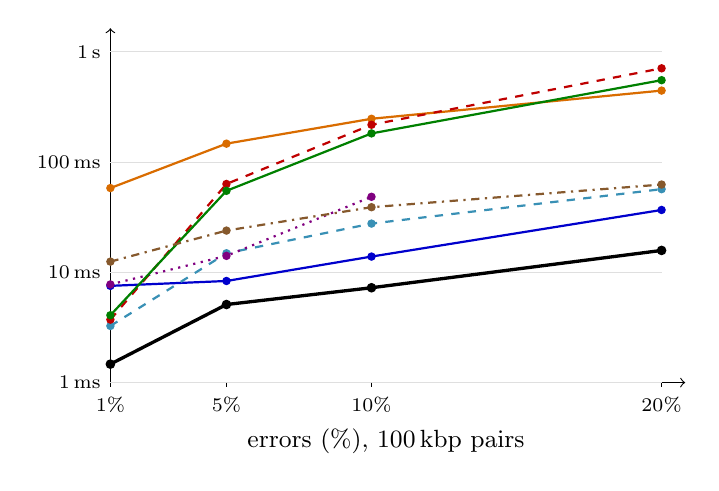
\begin{tikzpicture}
\draw[->] (0,0) -- (7.30,0);
\draw[->] (0,0) -- (0,4.50);
\draw[gray!25] (0,0.000) -- (7.00,0.000); \node[left,font=\scriptsize] at (0,0.000) {1\,ms};
\draw[gray!25] (0,1.400) -- (7.00,1.400); \node[left,font=\scriptsize] at (0,1.400) {10\,ms};
\draw[gray!25] (0,2.800) -- (7.00,2.800); \node[left,font=\scriptsize] at (0,2.800) {100\,ms};
\draw[gray!25] (0,4.200) -- (7.00,4.200); \node[left,font=\scriptsize] at (0,4.200) {1\,s};
\draw (0.000,0) -- (0.000,-0.06) node[below,font=\scriptsize] {1\%};
\draw (1.474,0) -- (1.474,-0.06) node[below,font=\scriptsize] {5\%};
\draw (3.316,0) -- (3.316,-0.06) node[below,font=\scriptsize] {10\%};
\draw (7.000,0) -- (7.000,-0.06) node[below,font=\scriptsize] {20\%};
\node[font=\small] at (3.50,-0.75) {errors (\%), 100\,kbp pairs};
\draw[dinara] plot coordinates {(0.000,0.234) (1.474,0.991) (3.316,1.204) (7.000,1.678)};
\draw[dinara,solid,fill=.] (0.000,0.234) circle (1.1pt);
\draw[dinara,solid,fill=.] (1.474,0.991) circle (1.1pt);
\draw[dinara,solid,fill=.] (3.316,1.204) circle (1.1pt);
\draw[dinara,solid,fill=.] (7.000,1.678) circle (1.1pt);
\draw[apafull] plot coordinates {(0.000,1.228) (1.474,1.290) (3.316,1.600) (7.000,2.192)};
\draw[apafull,solid,fill=.] (0.000,1.228) circle (1.1pt);
\draw[apafull,solid,fill=.] (1.474,1.290) circle (1.1pt);
\draw[apafull,solid,fill=.] (3.316,1.600) circle (1.1pt);
\draw[apafull,solid,fill=.] (7.000,2.192) circle (1.1pt);
\draw[apasimple] plot coordinates {(0.000,0.719) (1.474,1.642) (3.316,2.019) (7.000,2.456)};
\draw[apasimple,solid,fill=.] (0.000,0.719) circle (1.1pt);
\draw[apasimple,solid,fill=.] (1.474,1.642) circle (1.1pt);
\draw[apasimple,solid,fill=.] (3.316,2.019) circle (1.1pt);
\draw[apasimple,solid,fill=.] (7.000,2.456) circle (1.1pt);
\draw[apa] plot coordinates {(0.000,1.246) (1.474,1.609) (3.316,2.359)};
\draw[apa,solid,fill=.] (0.000,1.246) circle (1.1pt);
\draw[apa,solid,fill=.] (1.474,1.609) circle (1.1pt);
\draw[apa,solid,fill=.] (3.316,2.359) circle (1.1pt);
\draw[edlib] plot coordinates {(0.000,2.470) (1.474,3.034) (3.316,3.350) (7.000,3.708)};
\draw[edlib,solid,fill=.] (0.000,2.470) circle (1.1pt);
\draw[edlib,solid,fill=.] (1.474,3.034) circle (1.1pt);
\draw[edlib,solid,fill=.] (3.316,3.350) circle (1.1pt);
\draw[edlib,solid,fill=.] (7.000,3.708) circle (1.1pt);
\draw[biwfa] plot coordinates {(0.000,0.799) (1.474,2.522) (3.316,3.274) (7.000,3.991)};
\draw[biwfa,solid,fill=.] (0.000,0.799) circle (1.1pt);
\draw[biwfa,solid,fill=.] (1.474,2.522) circle (1.1pt);
\draw[biwfa,solid,fill=.] (3.316,3.274) circle (1.1pt);
\draw[biwfa,solid,fill=.] (7.000,3.991) circle (1.1pt);
\draw[wfa] plot coordinates {(0.000,0.855) (1.474,2.435) (3.316,3.164) (7.000,3.840)};
\draw[wfa,solid,fill=.] (0.000,0.855) circle (1.1pt);
\draw[wfa,solid,fill=.] (1.474,2.435) circle (1.1pt);
\draw[wfa,solid,fill=.] (3.316,3.164) circle (1.1pt);
\draw[wfa,solid,fill=.] (7.000,3.840) circle (1.1pt);
\draw[quicked] plot coordinates {(0.000,1.536) (1.474,1.930) (3.316,2.227) (7.000,2.515)};
\draw[quicked,solid,fill=.] (0.000,1.536) circle (1.1pt);
\draw[quicked,solid,fill=.] (1.474,1.930) circle (1.1pt);
\draw[quicked,solid,fill=.] (3.316,2.227) circle (1.1pt);
\draw[quicked,solid,fill=.] (7.000,2.515) circle (1.1pt);
\end{tikzpicture}}\end{minipage}\hfill\begin{minipage}{0.49\textwidth}\centering\textbf{b}\par\resizebox{\linewidth}{!}{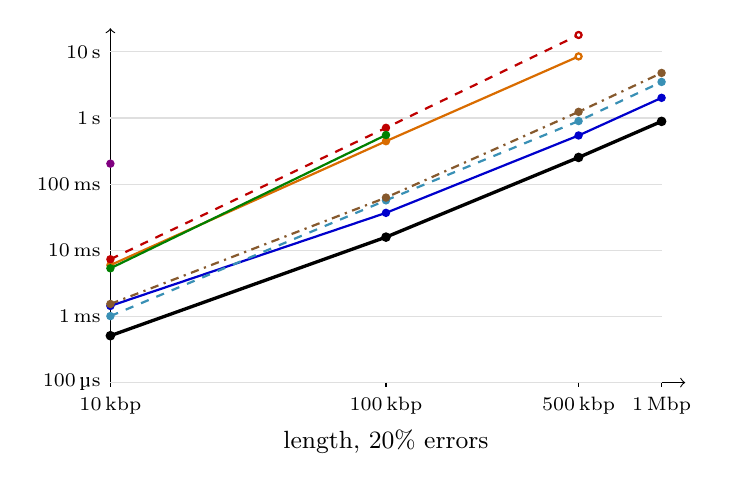
\begin{tikzpicture}
\draw[->] (0,0) -- (7.30,0);
\draw[->] (0,0) -- (0,4.50);
\draw[gray!25] (0,0.000) -- (7.00,0.000); \node[left,font=\scriptsize] at (0,0.000) {100\,\textmu s};
\draw[gray!25] (0,0.840) -- (7.00,0.840); \node[left,font=\scriptsize] at (0,0.840) {1\,ms};
\draw[gray!25] (0,1.680) -- (7.00,1.680); \node[left,font=\scriptsize] at (0,1.680) {10\,ms};
\draw[gray!25] (0,2.520) -- (7.00,2.520); \node[left,font=\scriptsize] at (0,2.520) {100\,ms};
\draw[gray!25] (0,3.360) -- (7.00,3.360); \node[left,font=\scriptsize] at (0,3.360) {1\,s};
\draw[gray!25] (0,4.200) -- (7.00,4.200); \node[left,font=\scriptsize] at (0,4.200) {10\,s};
\draw (0.000,0) -- (0.000,-0.06) node[below,font=\scriptsize] {10\,kbp};
\draw (3.500,0) -- (3.500,-0.06) node[below,font=\scriptsize] {100\,kbp};
\draw (5.946,0) -- (5.946,-0.06) node[below,font=\scriptsize] {500\,kbp};
\draw (7.000,0) -- (7.000,-0.06) node[below,font=\scriptsize] {1\,Mbp};
\node[font=\small] at (3.50,-0.75) {length, 20\% errors};
\draw[dinara] plot coordinates {(0.000,0.595) (3.500,1.847) (5.946,2.859) (7.000,3.317)};
\draw[dinara,solid,fill=.] (0.000,0.595) circle (1.1pt);
\draw[dinara,solid,fill=.] (3.500,1.847) circle (1.1pt);
\draw[dinara,solid,fill=.] (5.946,2.859) circle (1.1pt);
\draw[dinara,solid,fill=.] (7.000,3.317) circle (1.1pt);
\draw[apafull] plot coordinates {(0.000,0.973) (3.500,2.155) (5.946,3.138) (7.000,3.616)};
\draw[apafull,solid,fill=.] (0.000,0.973) circle (1.1pt);
\draw[apafull,solid,fill=.] (3.500,2.155) circle (1.1pt);
\draw[apafull,solid,fill=.] (5.946,3.138) circle (1.1pt);
\draw[apafull,solid,fill=.] (7.000,3.616) circle (1.1pt);
\draw[apasimple] plot coordinates {(0.000,0.844) (3.500,2.314) (5.946,3.321) (7.000,3.818)};
\draw[apasimple,solid,fill=.] (0.000,0.844) circle (1.1pt);
\draw[apasimple,solid,fill=.] (3.500,2.314) circle (1.1pt);
\draw[apasimple,solid,fill=.] (5.946,3.321) circle (1.1pt);
\draw[apasimple,solid,fill=.] (7.000,3.818) circle (1.1pt);
\draw[apa] plot coordinates {(0.000,2.780)};
\draw[apa,solid,fill=.] (0.000,2.780) circle (1.1pt);
\draw[edlib] plot coordinates {(0.000,1.491) (3.500,3.065) (5.946,4.142)};
\draw[edlib,solid,fill=.] (0.000,1.491) circle (1.1pt);
\draw[edlib,solid,fill=.] (3.500,3.065) circle (1.1pt);
\draw[edlib,solid,fill=white] (5.946,4.142) circle (1.1pt);
\draw[biwfa] plot coordinates {(0.000,1.566) (3.500,3.235) (5.946,4.414)};
\draw[biwfa,solid,fill=.] (0.000,1.566) circle (1.1pt);
\draw[biwfa,solid,fill=.] (3.500,3.235) circle (1.1pt);
\draw[biwfa,solid,fill=white] (5.946,4.414) circle (1.1pt);
\draw[wfa] plot coordinates {(0.000,1.451) (3.500,3.144)};
\draw[wfa,solid,fill=.] (0.000,1.451) circle (1.1pt);
\draw[wfa,solid,fill=.] (3.500,3.144) circle (1.1pt);
\draw[quicked] plot coordinates {(0.000,0.998) (3.500,2.349) (5.946,3.438) (7.000,3.932)};
\draw[quicked,solid,fill=.] (0.000,0.998) circle (1.1pt);
\draw[quicked,solid,fill=.] (3.500,2.349) circle (1.1pt);
\draw[quicked,solid,fill=.] (5.946,3.438) circle (1.1pt);
\draw[quicked,solid,fill=.] (7.000,3.932) circle (1.1pt);
\end{tikzpicture}}\end{minipage}
\par\medskip\resizebox{\linewidth}{!}{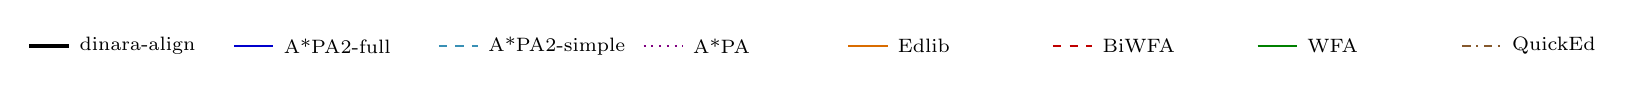
\begin{tikzpicture}[font=\scriptsize]
\draw[dinara] (0.00,0) -- (0.50,0) node[right,black] {dinara-align};
\draw[apafull] (2.60,0) -- (3.10,0) node[right,black] {A*PA2-full};
\draw[apasimple] (5.20,0) -- (5.70,0) node[right,black] {A*PA2-simple};
\draw[apa] (7.80,0) -- (8.30,0) node[right,black] {A*PA};
\draw[edlib] (10.40,0) -- (10.90,0) node[right,black] {Edlib};
\draw[biwfa] (13.00,0) -- (13.50,0) node[right,black] {BiWFA};
\draw[wfa] (15.60,0) -- (16.10,0) node[right,black] {WFA};
\draw[quicked] (18.20,0) -- (18.70,0) node[right,black] {QuickEd};
\end{tikzpicture}}
\caption{Unit-cost alignment of QuickEd's simulated pairs, mean time per alignment on a logarithmic scale. (a) 100~kbp pairs by error rate. (b) Pairs at 20\% errors by length; lines end where a tool completed no pair within 30~s or the 8 GiB limit stopped it, and hollow points mark tools that completed only some pairs. BSAlign and KSW2 are left out for legibility; their times are in the repository's benchmark tables. dinara-align had the lowest mean time at every length and error rate.}\label{fig:sweeps}
\end{figure*}

An alignment of an ultra-long read increased peak memory by at most 48 MiB, against 81 MiB for A*PA2-full, and of a 1~Mbp pair at 20\% errors by at most 123 MiB, against 184 MiB (Supplementary Table S7). This growth includes the seed heuristic and the band; the stored tile boundaries stayed within the default limit of 80 MiB (Section 3.7). QuickEd stayed near 25 MiB. On short reads dinara-align's peak was higher than the others' (Table~\ref{tab:unit}): the Mojo runtime and the sample, read whole, take about 13 MiB.

\section{Discussion}

dinara-align was the fastest exact aligner compared on every dataset at unit costs, and at gap-affine costs on every dataset that any tool completed, tied with WFA on the Illumina reads. This is consistent with choosing an algorithm for each pair: no single engine was fastest across these workloads, and since every engine is exact, choosing never forfeits the guarantee or changes the alignment. Three observations stand out. First, each technique paid where its engine does the work (Supplementary Table S2): on the ultra-long reads, switching off direct neighbour construction, which reduces work outside the inner loop, slowed alignment by 9 and 16\%, more than either change to the loop itself (at most 5\%), while the interleaved groups paid most on the widest bands and gathered extension where diagonal transition does most of the work. Second, on short reads the work that does not depend on the pair dominates: a 250~bp alignment at gap-affine costs once took 5.2~\textmu s through a fresh call and 2.4~\textmu s through a reused aligner (Supplementary Table S1), so a benchmark should call every tool as its own runner does. Third, thresholds that encode a cost model become outdated as the code changes, and measuring them again belongs in the evaluation of any aligner that selects its algorithm by thresholds. Gap-affine alignment of ultra-long reads remains open: no tool completed an ont-500k read within 30~s. Where memory matters more than time, Edlib, QuickEd and BiWFA (15 to 29 MiB on ultra-long reads) use less than dinara-align's 64 MiB. The measured-work rule, the regrouped recurrence and the per-lane certificate do not depend on this implementation and apply to other wavefront, bit-parallel and inter-sequence aligners.

\subsection{Limitations}

\begin{enumerate}
  \item The evaluation covers one x86 processor with AVX-512, and single-thread latency except for the batches; the AVX2 and NEON configurations are not evaluated here.
  \item The evaluated samples also guided development: several changes were motivated and checked on the Illumina, HiFi and ont-500k-genvar samples, and some thresholds, in particular the AVX-512 gates for inexact seeds, were set on uniform 100~kbp pairs like those of Fig.~\ref{fig:sweeps}a, so results on unseen data may be less favourable.
  \item The ultra-long and the largest simulated sets were sampled to four pairs. The three rounds were timed from one build, while on the Skylake-X running times varied by up to a third between builds that left the code involved unchanged (Supplementary Table S2), so margins of less than about 10\% may not hold across builds.
  \item The Illumina, HiFi and PromethION reads come from one region of one chromosome each and exclude reads that minimap2 leaves more than a tenth clipped, such as those spanning structural variants.
  \item The ablation switches off one technique at a time, so it does not separate their interactions.
\end{enumerate}

\subsection{Future work}

\begin{enumerate}
  \item a cheap upper bound on the distance: with the true distance supplied by an oracle, starting band doubling at it saves up to 27\% on 100~kbp pairs at 20\% errors, but starting 15\% above it loses up to 23\% on ultra-long reads, whereas capping the bound at an upper bound within 5\% of the distance saves up to 27\% on 1~Mbp pairs at 20\% (Supplementary Section S5);
  \item reusing computation across band-doubling rounds, as in the incremental doubling of A*PA2, once its exactness for these tiles is proven;
  \item faster construction of the seed heuristic, whose scalar lookups dominate on long divergent pairs, and a seed heuristic for gap-affine costs, at which no tool completed a 1~Mbp pair beyond 1\% errors;
  \item measurements on further processors, and an evaluation of the GPU kernels the library provides for batches (Supplementary Section S1.5).
\end{enumerate}

\section*{Author contributions}
Konstantinos Kyriakidis (Conceptualization [lead], Methodology [lead], Software [lead], Validation [lead], Formal analysis [lead], Investigation [lead], Data curation [lead], Visualization [lead], Writing—original draft [lead]), Benedict Paten (Supervision [lead], Writing—review \& editing [equal]).

\section*{Supplementary data}
Supplementary data are available at \emph{Bioinformatics} online.

\section*{Conflict of interest}
None declared.

\section*{Funding}
This work received no specific funding.

\section*{Data availability}
The software, benchmark harness and the commits of every compared tool are available at \url{https://github.com/kokyriakidis/dinara-align}. The benchmarks are reproduced by \texttt{pixi run bench} (unit and \texttt{-{}-affine} costs), \texttt{bench-modes}, \texttt{bench-batch} and \texttt{bench-ablation}. Release builds target the baseline processor of each platform; the AVX-512 code paths require a build for the host processor.

\bibliographystyle{oup-abbrvnat}
\bibliography{references}
\end{document}
